\documentclass{article}
\usepackage[margin=1.5in]{geometry}
\usepackage{graphicx}
\usepackage{nameref}
\usepackage{siunitx}
\usepackage[utf8]{inputenc}
\usepackage[toc,page]{appendix}

\begin{document}

\title{Localization for FRC \\
  \large{A Term Report}
  }
\author{Jinan (Dorothy) Hu, Peter Mitrano, Kacper Puczydlowski, Nicolette Vere}

\maketitle{}

\section{Introduction}

Knowing the position and orientation of a mobile robot is critical to many tasks. For robots designed for high-speed gameplay, knowing the position and orientation allows the robot to perform complex autonomous behaviors such as shooting and retrieving game objects. In this report, we describe a system for determining the pose $(x, y, \theta)$ of a mobile robot in a cluttered environment. The environment we are interested in is the FIRST Robotics Competition (FRC). FRC is a challenging environment because the robots make rapid and aggressive maneuvers by human drivers for part of the time, and at other times are under complete autonomy. A successful localization system for FRC must handle up to six robots, occlusion from the playing field elements, unpredictable lighting, and frequent impacts. Our research suggests that there are at least five appropriate methods for localization: cameras and tags, radio and ultrasonic beacons, optical flow, and dead reckoning with encoders, and dead reckoning with an IMU. All of these methods have seen success in robot localization.

This report begins with a review of existing literature on indoor localization for mobile robots in the \nameref{related_work} section. The strengths and weaknesses of these existing methods are described in the \nameref{methods} section. The \nameref{experiments} section contains information on experiments we conducted, and the \nameref{conclusion} section details our plan moving forward.

\section{Related Work} \label{related_work}

Robot localization has been studied for decades. Overall, the problem of localizing a mobile robot can be viewed as accurately measure the absolute distance to known landmarks, or by measuring the changes in position over time. We will henceforth refer to these two ideas as global and local pose estimation. Some of the high level techniques for robot localization are: measuring range at various points around the robot and matching these readings to a map, measuring time of flight or difference of time of arrival to calculate distance to known locations, recognizing landmarks in some modality and computing pose relative to those landmarks, and measuring changes in pose and accumulating these changes over time. There are different sensors that can be used for each of these techniques, such as laser range finders, ultrasonic, cameras, inertial measurement units (IMU), encoders, radio, visible light, and human-audible sound. Although there are a tremendous number of possible methods for robot localization, there are a few which have received the most attention and shown the most success. These include:
\begin{itemize}
    \item Lidar mapping
    \item Ultrasonic mappping
    \item IMU and Encoders fusion
    \item Infrared or Radio and Ultrasonic beacons
    \item cameras with visually identifiable tags
    \item Optical flow mice and cameras
    \item Stereo vision and depth cameras
\end{itemize}

In our research, we learned how these seven techniques work and found descriptions and implementations in order to evaluate them. These descriptions and implementations are described in this section with the purpose of demonstrating a thorough literature review and of providing background information to the reader.

**Here we will go over all the papers we read and sources we talked to. Explain what if any of our approach is novel and what is built on existing approaches.

Beacon systems have been used many times with success in the literature. Generally, these systems ultrasound and or radio as a medium and either signal strength, phase shift, or time to measure distance to the beacons. Among radio systems, the system in \cite{bahl_radar:_2000} identified the location of people moving around buildings using signal strength in the 2.4gHz band received at three or more beacons, and they report accuracy of a few meters with an update rate of at most four times per second. The systems described in \cite{digiampaolo_mobile_2014} uses passive RFID tags on the ceiling and an RFID transmitter on the robot, and report an accuracy of 4\si{\centi\meter} within a 5\si{\square\meter}. Another RFID system \cite{saab_standalone_2011} also uses signal strength to RFID, and reports accuracies for various configurations ranging from 1\si{\centi\meter} to 3\si{\meter}. These RFID systems require readers that cost over \$500. There are also countless localization systems that use standard wireless networks. A comprehensive survey of these systems can be found in \cite{liu_survey_2007}. Systems that use signal strength in standard wireless LAN networks have achieved up to 10\si{\centi\meter} accuracy and hundreds of updates per second. Another radio beacon solution is to substitute single-frequency radio with Ultra-wideband radio. These systems can achieve centimeter level accuracy, but they use obscure or custom made transmitters and receivers that cost in the hundreds of dollars \cite{noauthor_dart_nodate} \cite{noauthor_pozyx_nodate}.

Many beacon systems use the speed difference between sound and electromagnetic waves to measure system. Systems like \cite{smith_tracking_2004} \cite{ward_new_1997} \cite{kim_advanced_2008} send radio pulses followed by ultrasonic pulses. Nodes in the network us the difference in arrival time of these two signals to measure distance. Alternately, some systems use infrared pulses in place of radio \cite{ghidary_new_1999} \cite{yucel_development_2012}. These systems are inexpensive, and report accuracy of between 2 and 14\si{\centi\meter}.

\section{Evaluation of Localization Techniques} \label{methods}

Each of the techniques presented thus far have strengths and weaknesses, and it is unlikely that any one technique would be sufficient. This is the motivation for combining multiple techniques. To do so effectively, we compare each technique so as to mitigate the errors in any one technique. The five

Optical flow gives us accurate angle measurements and fast updates that are relative to our current position. Like all camera based solutions, the vibration of the robot will likely makes this technique difficult. However, cameras are the most widely used sensor according to our survey of FRC students and alumni.
The camera also doubles as a sensor for matrix tags, which give us accurate position estimates in the global frame. This is complemented by beacons, which update more slowly, but are not effected by occlusion and is robust to vibration.

\section{Experimental Results} \label{experiments}

**How did we test ArUco tags, IMUs, Optimal Flow. What results? Be specific. Include any relevant charts or equations.

We demonstrated radio communication between two microcontrollers and tested the effect of distance and occlusion.

\section{Conclusion} \label{conclusion}

Based on the extensive literature review and the few preliminary experiments we've conducted, we eliminated our initial list of possible techniques down to the following five:
\begin{enumerate}
    \item Radio and ultrasonic beacons
    \item IMU
    \item Drive wheel encoders
    \item Optical flow
    \item Camera with matrix tags
\end{enumerate}

We have found examples of each of these techniques being used successfully, and in many cases have verified that they satisfy our criteria for accuracy, precision, update rate, and accessibility criteria. We are confident that any combination of these methods would work. Nonetheless, it is unreasonable to attempt to use all of these methods in the time frame of this project, and therefore we have decided to move forward with beacons, optical flow, and matrix tags. These techniques are complementary in their sources of error, and together we believe they will make a robust localization system.

% TODO: explain the parts we know in detail, like the proposed beacon protocol

% TODO: Setup appendix for things like the survey

\begin{appendices}
  \chapter{Appendix A} \\

  Survery Responses

  \begin{figure}
    \centering
    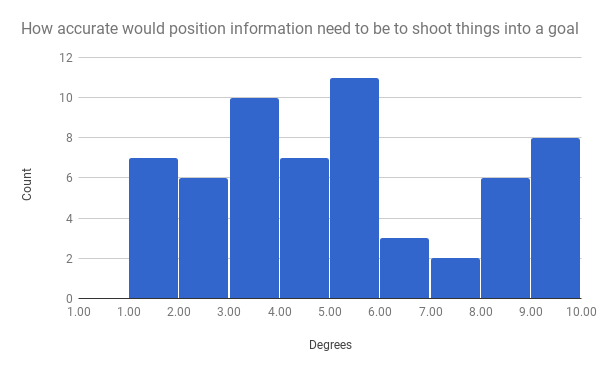
\includegraphics[width=1\linewidth]{./survey_angle.png}
    \label{fig:survey_angle}
  \end{figure}

  \begin{figure}
    \centering
    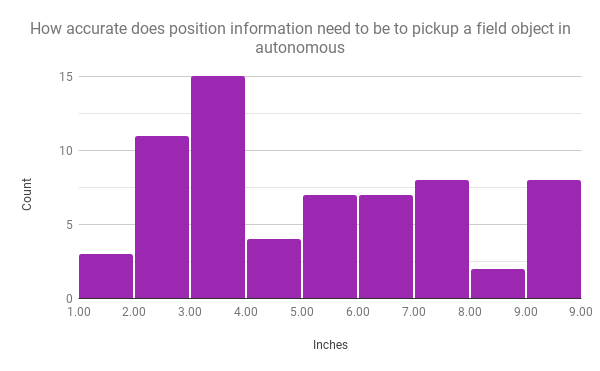
\includegraphics[width=1\linewidth]{./survey_position.png}
    \label{fig:survey_position}
  \end{figure}

  \begin{figure}
    \centering
    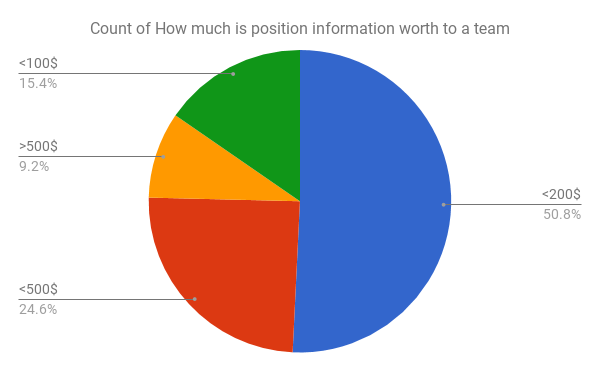
\includegraphics[width=1\linewidth]{./survey_worth.png}
    \label{fig:survey_worth}
  \end{figure}

\end{appendices}


\bibliographystyle{plain}
\bibliography{phil-mqp}
\end{document}
